 \documentclass{article}

% Language setting
% Replace `english' with e.g. `spanish' to change the document language
\usepackage[portuguese]{babel}

% Set page size and margins
% Replace `letterpaper' with `a4paper' for UK/EU standard size
\usepackage[letterpaper,top=2cm,bottom=2cm,left=3cm,right=3cm,marginparwidth=1.75cm]{geometry}

% Useful packages
\usepackage{amsmath}
\usepackage{graphicx}
\usepackage[colorlinks=true, allcolors=blue]{hyperref}
\usepackage{listings}
\usepackage{xcolor}

\definecolor{codegreen}{rgb}{0,0.6,0}
\definecolor{codegray}{rgb}{0.5,0.5,0.5}
\definecolor{codepurple}{rgb}{0.58,0,0.82}
\definecolor{backcolour}{rgb}{0.95,0.95,0.92}

\lstdefinestyle{mystyle}{
    backgroundcolor=\color{backcolour},   
    commentstyle=\color{codegreen},
    keywordstyle=\color{magenta},
    numberstyle=\tiny\color{codegray},
    stringstyle=\color{codepurple},
    basicstyle=\ttfamily\footnotesize,
    breakatwhitespace=false,         
    breaklines=true,                 
    captionpos=b,                    
    keepspaces=true,                 
    numbers=left,                    
    numbersep=5pt,                  
    showspaces=false,                
    showstringspaces=false,
    showtabs=false,                  
    tabsize=2
}

\lstset{style=mystyle}

\title{TP2 - Redes de Computadores}
\author{Francisco Ferreira - a100660\\Júlio Pinto - a100742\\Rui Lopes - a100643}

\begin{document}
\maketitle
\tableofcontents

\pagebreak
\bigskip

\section{Exercício 3}

Nas seguintes questões, foi utilizado o seguinte filtro no Wireshark:

\begin{figure}[h]
    \lstinline{(ip.src == 192.168.1.35 && ip.dst == 193.137.9.171) || (ip.src == 193.137.9.171 && ip.dst == 192.168.1.35)}
\end{figure}
 \noindent Assim, no output do Wireshark, apenas aparecerão pacotes enviados desde a minha máquina até ao servidor onde se encontra o domínio alunos.uminho.pt e vice-versa.

\subsection{Alínea 1)}

Anote os endereços MAC de origem e de destino da trama capturada. Identifique a que sistemas se referem. Justifique.


\subsubsection{Resposta alínea 1)}

O endereço MAC de origem é 50:76:af:15:77:a0 e o de destino é 86:0b:7c:bc:d7:83. O endereço de origem refere-se à máquina nativa utilizada e o de destino refere-se ao router de acesso/default gateway. Isto pois, ao contrário do nível protocolar IP, o nível de ligação lógica vai recalculando salto-a-salto o endereço MAC destino contido na trama a ser enviada - parando apenas quando este coincidir com o endereço IP destino (neste caso 193.137.9.171).

\begin{figure}[h!]
    \centering
    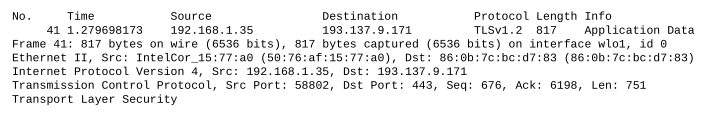
\includegraphics[width=\textwidth]{ex1.png}
\end{figure}

\subsection{Alínea 2)}

Qual o valor hexadecimal do campo Type da trama Ethernet? O que significa?

\subsubsection{Resposta alínea 2)}

Também conhecido como "EtherType", este campo é utilizado para indicar qual é o protocolo encapsulado pela trama. O valor 0x0800 indica que é IPv4. 0x0806 seria ARP, por exemplo. (Para mais valores consultar: \href{https://en.wikipedia.org/wiki/EtherType}{EtherType - Wikipedia}

\pagebreak

\subsection{Alínea 3)}

Quantos bytes são usados no encapsulamento protocolar, i.e. desde o início da trama até ao início dos dados do nível
aplicacional (Application Data Protocol: http-over-tls, no caso de HTTPS)? Calcule e indique, em percentagem, a
sobrecarga (overhead) introduzida pela pilha protocolar.

\subsubsection{Resposta alínea 3)}

Neste caso, "entram vários protocolos em jogo": IPv4, TCP e Ethernet. O primeiro contém um cabeçalho de 20 bytes (tal como foi estudado no trabalho prático anterior), o segundo contém um cabeçalho de 32 bytes (conferir imagem anexada) e o terceiro contém um cabeçalho de 14 bytes. 
Se somados, totalizam 66 bytes. Uma vez que o tamanho total do pacote é de 817 bytes, isto implica uma percentagem de aproximadamente 8.08%.

\begin{figure}[h!]
    \centering
    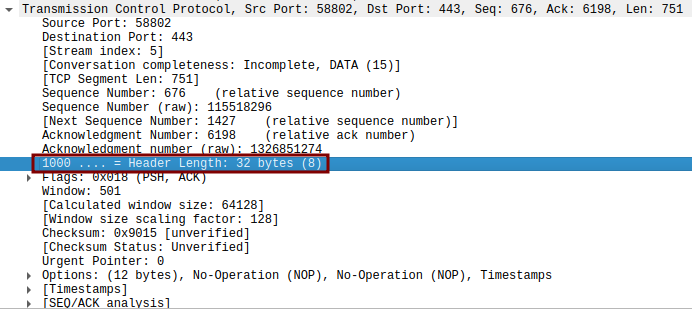
\includegraphics[width=\textwidth]{ex3-3.png}
\end{figure}

\subsection{Alínea 4)}

Qual é o endereço Ethernet da fonte? A que sistema de rede corresponde? Justifique.

\subsubsection{Resposta alínea 4)}

O endereço Ethernet da fonte é 86:0b:7c:bc:d7:83. Este endereço é exatamente o mesmo que, na trama capturada na alínea anterior, era o endereço MAC de destino - router de acesso/default gateway. Isto acontece, pois este é o último salto no envio de pacotes até à máquina nativa.
`

\pagebreak
\subsection{Alínea 5)}

Qual é o endereço MAC do destino? A que sistema (host) corresponde?

\subsubsection{Resposta alínea 5)}

O endereço MAC do destino é 50:76:af:15:77:a0. Este endereço corresponde à máquina nativa utilizada. Novamente, este endereço corresponde ao endereço MAC origem, na trama capturada na alínea anterior.

\subsection{Alínea 6)}

Atendendo ao conceito de encapsulamento protocolar, identifique os vários protocolos contidos na trama recebida.
Justifique, indicando em que campos dos cabeçalhos capturados se baseou.

\subsubsection{Resposta alínea 6)}

Antes de mais, é essencial perceber como funciona uma pilha protocolar. Numa pilha protocolar existem várias camadas que constituem uma espécie de hierarquia - uma camada fornece serviços à camada diretamente acima e utiliza serviços da camada diretamente abaixo. Neste caso, é possível perceber que existem três camadas: camada de transporte (TCP), camada de rede (IP) e camada de ligação lógica (Ethernet). Todas contribuem para que exista um certo overhead (já calculado na alínea anterior).


\section{Exercício 4}
\textbf{Departamento A:} 192.168.12.X/25 
\textbf{Departamento B:} 192.168.140.X/25

\begin{figure}[h!]
    \centering
    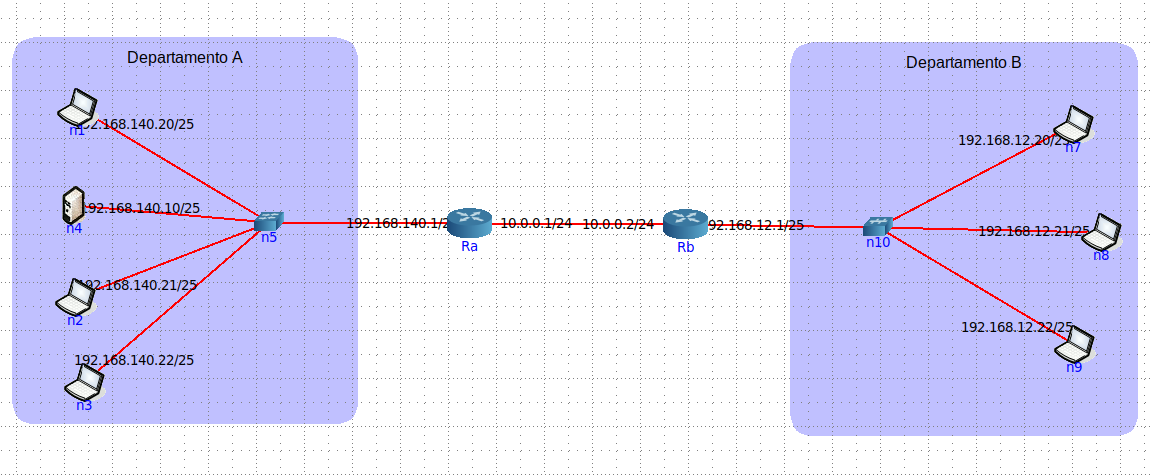
\includegraphics[width=\textwidth]{topologia-4.png}
\end{figure}

\bigskip
\subsection{Alínea 1)}

Abra uma consola no PC onde efetuou o ping. Observe o conteúdo da tabela ARP com o comando arp -a.

\subsection{Alínea 1.a)}

Com a ajuda do manual ARP (man arp), interprete o significado de cada uma das colunas da tabela

\subsubsection{Resposta alínea 1.a)}

\begin{lstlisting}
> arp -a
? (192.168.140.1) at 00:00:00:aa:00:00 [ether] on eth0
\end{lstlisting}

\noindent A primeira coluna refere-se ao nome da entrada (neste caso a entrada não tem um nome definido); A segunda coluna refere-se ao endereço IP destino; A terceira coluna refere-se ao endereço MAC destino correspondente ao IP destino; A quarta e última coluna refere-se à interface pela qual devemos encaminhar o tráfego

\subsection{Alínea 1.b)}

Indique, justificando, qual o equipamento da intranet em causa que poderá apresentar a maior tabela ARP em termos de número de entradas.

\subsubsection{Resposta alínea 1.b)}

O Ra (router de acesso A) é o equipamento que poderá apresentar a maior tabela ARP. Isto pois, este encontra-se ligado tanto ao Rb (router de acesso B) como aos 4 dispositivos presentes na sua rede - totalizando 5 entradas na tabela ARP (demonstração em baixo)

\begin{lstlisting}
> arp -a
? (192.168.140.10) at 00:00:00:aa:00:05 [ether] on eth0
? (192.168.140.21) at 00:00:00:aa:00:06 [ether] on eth0
? (192.168.140.22) at 00:00:00:aa:00:07 [ether] on eth0
? (192.168.140.20) at 00:00:00:aa:00:04 [ether] on eth0
? (10.0.0.2) at 00:00:00:aa:00:03 [ether] on eth1
\end{lstlisting}

\subsection{Alínea 2)}

Observe a trama Ethernet que contém a mensagem com o pedido ARP (ARP Request).

\subsection{Alínea 2.a)}

Qual é o valor hexadecimal dos endereços MAC origem e destino? Como interpreta e justifica o endereço destino
usado?

\subsubsection{Resposta alínea 2.a)}

O valor hexadecimal do endereço MAC origem é 00:00:00:aa:00:04 (referente ao dispositivo que efetuou o ping). O valor hexadecimal do endereço MAC destino é ff:ff:ff:ff:ff:ff, o que significa que foi realizado um broadcast. Isto dá-se pois o endereço MAC destino não é conhecido, então envia-se um ARP request para todos os dispositivos na rede local - cada um deles, depois de receber o pedido, verifica se o endereço IP é o seu e, em caso afirmativo, envia de volta o endereço MAC correspondente.

\begin{figure}[h]
    \centering
    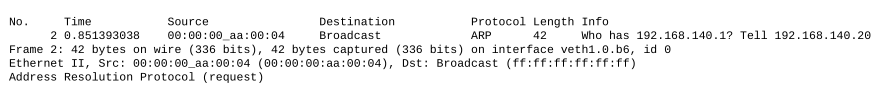
\includegraphics[width=\textwidth]{4-2a.png}
\end{figure}

\subsection{Alínea 2.b)}

Qual o valor hexadecimal do campo Tipo da trama Ethernet? O que indica?

\subsubsection{Resposta alínea 2.b)}

O valor hexadecimal é 0x0806, que indica tratar-se um pedido ARP.

\pagebreak


\subsection{Alínea 2.c)}

Observando a mensagem ARP, como pode saber que se trata efetivamente de um pedido ARP? Refira duas
formas distintas de obter essa informação.

\subsubsection{Resposta alínea 2.c)}

Exatamente pelos pontos anteriormente descritos. O endereço MAC destino ser ff:ff:ff:ff:ff:ff e o tipo do pedido ser ARP.


\subsection{Alínea 2.d)}

Explicite, em linguagem comum, que tipo de pedido ou pergunta é feita pelo host de origem à rede?

\subsubsection{Resposta alínea 2.d)}

O host de origem pergunta quem tem o IPv4 192.168.140.1 e pede também que a resposta seja enviada para o IPv4 192.168.140.20 (o seu, no caso).

\subsection{Alínea 3)}

Localize a mensagem ARP que é a resposta ao pedido ARP efetuado.

\subsection{Alínea 3.a)}

Qual o valor do campo ARP opcode? O que especifica?

\subsubsection{Resposta alínea 3.a)}

O valor do campo ARP opcode é 2. Este valor especifica que a mensagem é uma resposta ARP (ARP reply).
\begin{figure}[h]
    \centering
    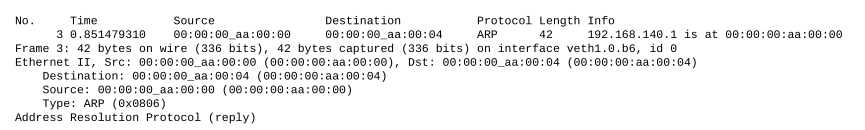
\includegraphics[width=\textwidth]{4-3a.png}
\end{figure}

\subsection{Alínea 3.b)}

Em que posição da mensagem ARP está a resposta ao pedido ARP efetuado?

\subsubsection{Resposta alínea 3.b)}

A resposta ao pedido efetuado encontra-se em "Sender MAC address" (tal como é possível verificar pela imagem em baixo).
\begin{figure}[h]
    \centering
    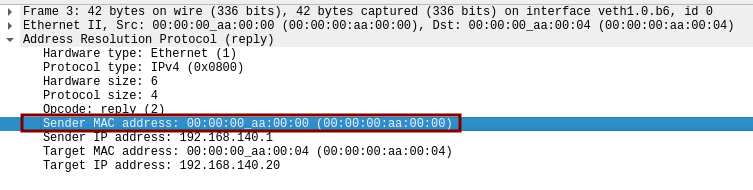
\includegraphics[width=\textwidth]{4-3b.png}
\end{figure}

\subsection{Alínea 3.c)}

Identifique a que sistemas correspondem os endereços MAC de origem e de destino da trama em causa, recorrendo aos comandos ifconfig, netstat -rn e arp executados no PC selecionado.

\subsubsection{Resposta alínea 3.c)}

O endereço MAC origem corresponde ao endereço pedido pelo equipamento que enviou o ARP request. Já o endereço MAC destino corresponde ao equipamento que enviou o pedido. A primeira afirmação é facilmente justificado com a tabela ARP demonstrada em baixo e a segunda com a imagem, também em baixo.
\begin{lstlisting}
> arp
Address                  HWtype  HWaddress           Flags Mask            Iface
192.168.140.1            ether   00:00:00:aa:00:00   C                     eth0
\end{lstlisting}
\begin{figure}[h]
    \centering
    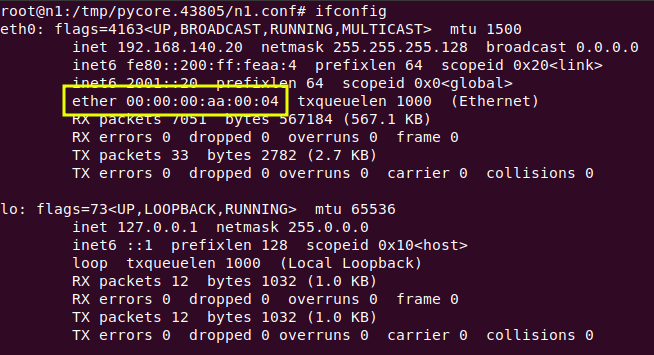
\includegraphics[width=\textwidth]{4-3c.png}
\end{figure}

\subsection{Alínea 3.d)}

Justifique o modo de comunicação (unicast vs. broadcast) usado no envio da resposta ARP (ARP Reply).

\subsubsection{Resposta alínea 3.d)}

A resposta ARP (ARP reply) é simplesmente um unicast, isto porque já é sabido o endereço MAC destino (exatamente o endereço MAC origem do pedido ARP).

\subsection{Alínea 4)}

Verifique se o ping feito ao segundo PC originou pacotes ARP. Justifique a situação observada.

\subsubsection{Resposta alínea 4)}

Não, o segundo ping não originou pacotes ARP. Isto pois, o tráfego que tem como destino outra rede, é enviado primeira para o router de acesso - cujo endereço MAC já é conhecido. Ou seja, não faz sentido perguntar qual é novamente.

\subsection{Alínea 5)}

Identifique na mensagem ARP os campos que permitem definir o tipo e o tamanho dos endereços das camadas de rede e de ligação lógica que se pretendem mapear. Justifique os valores apresentados nesses campos.

\subsubsection{Resposta alínea 5)}

No campo "Protocol type" é estabelecida a utilização do protocolo IPv4. No campo "Harware size" é definido que o hardware é compatível com endereços IPv6, mas o campo "Protocol size" vem confirmar que o protocolo utilizado é efetivamente IPv4, já que o seu valor é 4. 
\begin{figure}[h]
    \centering
    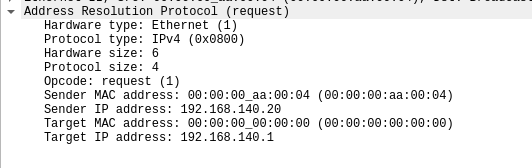
\includegraphics[width=\textwidth]{4-5.png}
\end{figure}

\subsection{Alínea 6)}
Na situação em que efetua um ping a um PC não local à sua sub-rede, esboce um diagrama em que indique claramente, e de forma cronológica, todas as mensagens ARP e ICMP trocadas, até à recepção da resposta ICMP do sistema destino (represente apenas os nós intervenientes). Assuma que todas as tabelas ARP se encontram inicialmente vazias.
\pagebreak

\subsubsection{Resposta alínea 6)}

\begin{figure}[h]
    \centering
    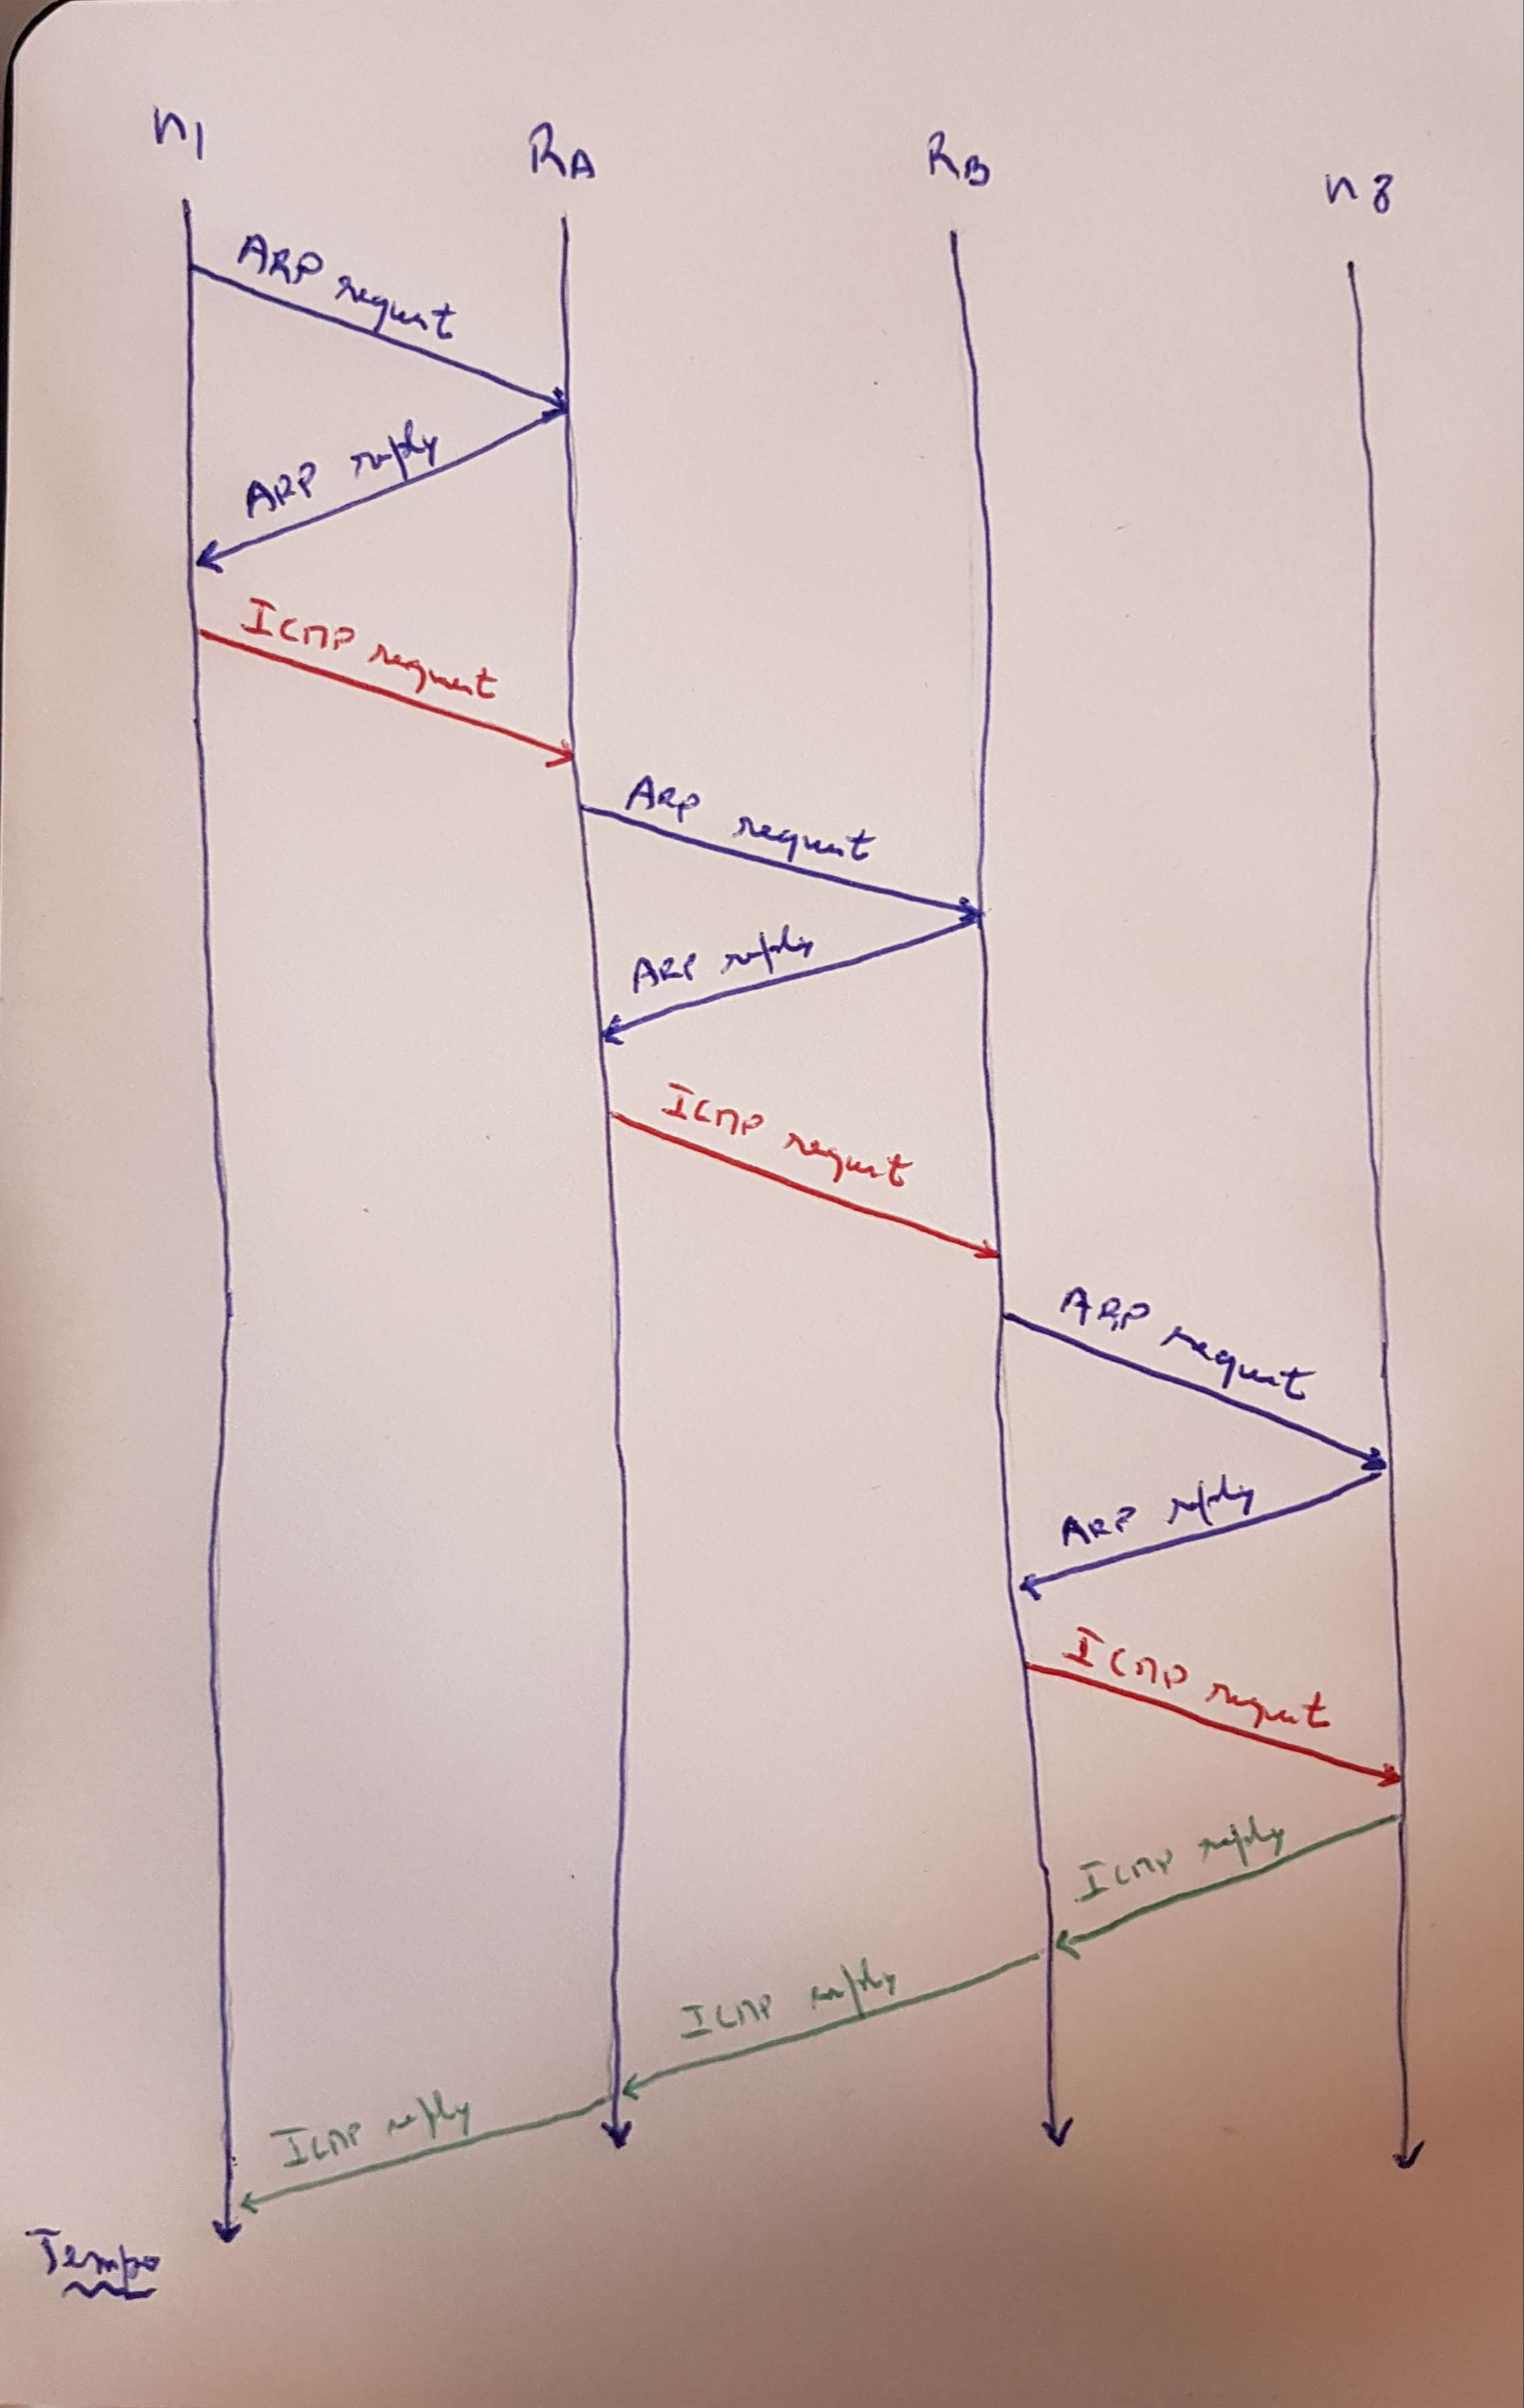
\includegraphics[height=15cm]{4-6.png}
\end{figure}


\pagebreak

\section{Exercício 5}

Considere a topologia de rede definida anteriormente.

\subsection{Alínea 1)}
Através da opção tcpdump, verifique e compare como flui o tráfego nas diversas interfaces dos vários dispositivos no departamento A (LAN comutada) e no departamento B (LAN partilhada) quando é gerado tráfego intra-departamento (por exemplo, através do comando ping). Que conclui?
Comente os resultados obtidos quanto à utilização de hubs e switches no contexto de controlar ou dividir domínios de colisão. Documente as suas observações e conclusões com base no tráfego observado/capturado.

\subsubsection{Resposta alínea 1)}

tcpdump em n4 após ping do n1 para o n2 (no departamento A, que utiliza um switch):
\begin{lstlisting}
> tcpdump
tcpdump: verbose output suppressed, use -v or -vv for full protocol decode
listening on eth0, link-type EN10MB (Ethernet), capture size 262144 bytes
14:08:37.575470 IP 192.168.140.1 > 224.0.0.5: OSPFv2, Hello, length 44
14:08:39.575517 IP 192.168.140.1 > 224.0.0.5: OSPFv2, Hello, length 44
14:08:41.575899 IP 192.168.140.1 > 224.0.0.5: OSPFv2, Hello, length 44

3 packets captured
3 packets received by filter
0 packets dropped by kernel
\end{lstlisting}

\noindent tcpdump em n8 após ping do n7 para o n9 (no departamento B, que utiliza um hub):
\begin{lstlisting}
> tcpdump
tcpdump: verbose output suppressed, use -v or -vv for full protocol decode
listening on eth0, link-type EN10MB (Ethernet), capture size 262144 bytes
14:10:37.932720 IP 192.168.12.1 > 224.0.0.5: OSPFv2, Hello, length 44
14:10:38.568102 IP 192.168.12.20 > 192.168.12.22: ICMP echo request, id 35, seq 1, length 64
14:10:38.568393 IP 192.168.12.22 > 192.168.12.20: ICMP echo reply, id 35, seq 1, length 64
14:10:39.578088 IP 192.168.12.20 > 192.168.12.22: ICMP echo request, id 35, seq 2, length 64
14:10:39.580117 IP 192.168.12.22 > 192.168.12.20: ICMP echo reply, id 35, seq 2, length 64
14:10:39.934667 IP 192.168.12.1 > 224.0.0.5: OSPFv2, Hello, length 44
14:10:40.581308 IP 192.168.12.20 > 192.168.12.22: ICMP echo request, id 35, seq 3, length 64
14:10:40.581683 IP 192.168.12.22 > 192.168.12.20: ICMP echo reply, id 35, seq 3, length 64
14:10:41.581283 IP 192.168.12.20 > 192.168.12.22: ICMP echo request, id 35, seq 4, length 64
14:10:41.581395 IP 192.168.12.22 > 192.168.12.20: ICMP echo reply, id 35, seq 4, length 64
14:10:41.938994 IP 192.168.12.1 > 224.0.0.5: OSPFv2, Hello, length 44

11 packets captured
11 packets received by filter
0 packets dropped by kernel
\end{lstlisting}

\noindent Olhando para os dois outputs do comando tcpdump é possível perceber uma clara diferença. Isto acontece porque no departamento A existe uma rede LAN comutada (switch) e no departamento B existe uma rede LAN partilhada (hub). 
Existem várias diferenças entre hubs e switches, sendo uma delas a forma como operam. Os hubs são dispositivos que reencaminham a trama que recebem por todas as interfaces que têm, criando uma difusão da mesma. Por outro lado, os switches possuem uma tabela de comutação que ajuda no envio das tramas que recebem precisamente para a interface apropriada. No entanto, caso um switch receba uma trama cujo endereço destino não se encontra na tabela, este difunde a trama por todas as interfaces (comportando-se como um hub, portanto).
Tendo em mente o dito anteriormente, é trivial perceber o porquê da diferença entre os outputs. Na LAN comutada (primeiro output), o tráfego entre os hosts n1 e n2 é corretamente encaminhado pelo switch, sem que o host n4 recebe também tráfego que não lhe diz respeito. De outro modo, na LAN partilhada (segundo output), o host n8, ainda que não envolvido diretamente no tráfego com destino ao host n9, também recebeu as tramas - isto pois, o hub encaminhou o tráfego por todas as suas interfaces.

\subsection{Alínea 2)}
Construa manualmente a tabela de comutação do switch do Departamento A, atribuindo números de porta à sua escolha.

\subsubsection{Resposta alínea 2)}

\begin{center}
\begin{tabular}{ |c |c| c| }
\hline
 Mac Address & Interface & TTL \\
\hline\hline
00:00:00:aa:00:04 & eth1 & 60 \\ [1ex] 
\hline
00:00:00:aa:00:05 & eth2 & 60 \\ [1ex]
\hline
00:00:00:aa:00:06 & eth3 & 60 \\ [1ex]
\hline
00:00:00:aa:00:07 & eth4 & 60  \\ [1ex]
\hline
\end{tabular}
\end{center}

\end{document}